\documentclass[11pt]{article}
\IfFileExists{acl.sty}{\usepackage[review]{acl}}{\usepackage[margin=1in]{geometry}}
\usepackage{booktabs}
\usepackage{graphicx}
\usepackage{microtype}
\usepackage{tikz}
\usetikzlibrary{arrows.meta,fit,positioning}
\title{ContextTrace: Evidence-Chain Forensics for Retrieval-Augmented Generation}
\author{Anonymous ARR submission}

\begin{document}
\maketitle
\begin{abstract}
Retrieval-augmented generation evaluators often reduce a trace to aggregate
quality scores, leaving engineers to reconstruct why an answer failed and what
to repair. ContextTrace is a local-first evaluator that maps claims through
retrieved evidence, citations, source conditions, and abstention behavior to
structured failure diagnoses. This draft defines the system, benchmark
protocol, and preregistered actionability study. All quantitative tables report
frozen pre-review evidence and identify review-pending results explicitly.
\end{abstract}

\section{Introduction}
RAG failures can arise from retrieval, evidence quality, citation alignment,
claim overreach, contradiction, or a missing abstention. Aggregate scores do
not identify which component should change. We study evidence-chain forensics:
the task of producing a traceable diagnosis from answer claims to supporting
or conflicting spans and then to a concrete failure class.

ContextTrace implements this task as a deterministic, local-first verification
pipeline. The intended contribution is not another scalar judge. It is an
inspectable diagnostic contract, an evaluation protocol that preserves
unsupported outputs as unavailable rather than imputing them, and a human
study designed to test whether the added structure improves repair decisions.

\section{Related Work}
RAG evaluation spans retrieval quality, answer faithfulness, context relevance,
and task-level correctness. Existing evaluator suites provide useful automatic
signals, but systems differ in the diagnostic fields they expose. Our matched
comparisons therefore score common outputs on identical case IDs and report
unsupported diagnostics as N/A. The final draft will position ContextTrace
against RAG evaluation, attribution, factuality, and debugging work using
verified primary-source citations only.

\section{Evidence-Chain Model}
An evidence chain links a query and generated answer to atomic claims,
retrieved contexts, citation edges, support or contradiction decisions,
localized spans, source conditions, and a failure diagnosis. Figure~\ref{fig:pipeline}
shows the contract, while Figure~\ref{fig:trace} gives a compact trace example.
This representation makes intermediate decisions serializable and auditable.

\begin{figure*}[t]
\centering
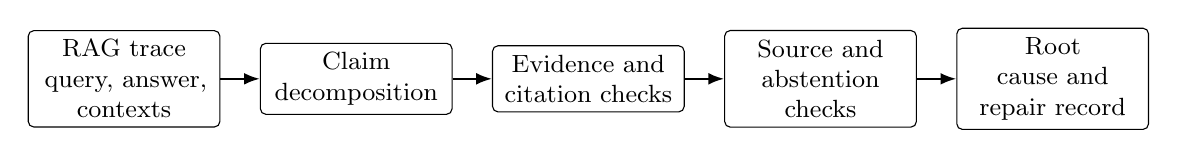
\begin{tikzpicture}[
  node distance=5mm and 5mm,
  box/.style={draw, rounded corners=2pt, align=center, minimum height=8mm, text width=22mm, font=\small},
  arrow/.style={-{Latex[length=2mm]}, thick}
]
\node[box] (trace) {RAG trace\\query, answer, contexts};
\node[box, right=of trace] (claims) {Claim\\decomposition};
\node[box, right=of claims] (evidence) {Evidence and\\citation checks};
\node[box, right=of evidence] (conditions) {Source and\\abstention checks};
\node[box, right=of conditions] (diagnosis) {Root cause and\\repair record};
\draw[arrow] (trace) -- (claims);
\draw[arrow] (claims) -- (evidence);
\draw[arrow] (evidence) -- (conditions);
\draw[arrow] (conditions) -- (diagnosis);
\end{tikzpicture}
\caption{ContextTrace production pipeline. Each stage emits a serializable
record used by downstream diagnosis and audit.}
\label{fig:pipeline}
\end{figure*}

\begin{figure}[t]
\centering
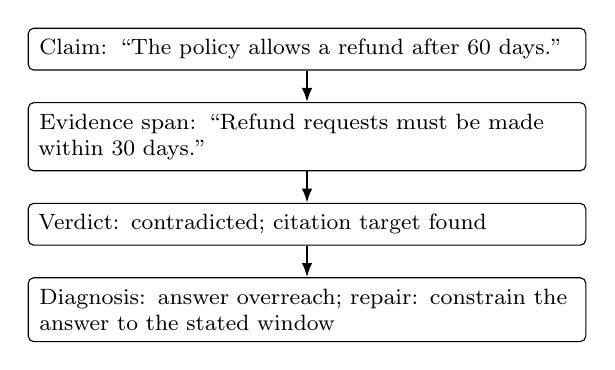
\begin{tikzpicture}[
  node distance=4mm,
  item/.style={draw, rounded corners=2pt, align=left, text width=68mm, font=\footnotesize, inner sep=4pt},
  arrow/.style={-{Latex[length=1.8mm]}, thick}
]
\node[item] (claim) {Claim: ``The policy allows a refund after 60 days.''};
\node[item, below=of claim] (span) {Evidence span: ``Refund requests must be made within 30 days.''};
\node[item, below=of span] (verdict) {Verdict: contradicted; citation target found};
\node[item, below=of verdict] (repair) {Diagnosis: answer overreach; repair: constrain the answer to the stated window};
\draw[arrow] (claim) -- (span);
\draw[arrow] (span) -- (verdict);
\draw[arrow] (verdict) -- (repair);
\end{tikzpicture}
\caption{Illustrative evidence-chain trace. The example describes the output
schema and is not a scored benchmark result.}
\label{fig:trace}
\end{figure}


\section{System}
The verifier normalizes a trace, decomposes its answer into claims, retrieves
candidate evidence spans, classifies claim support and contradiction, validates
citations, evaluates source trust and freshness when metadata are present, and
assigns a primary root cause. Profiles expose each module boundary so ablations
exercise the production code path rather than a separate research model.

The default path is offline and deterministic. Optional model-based evaluators
must pin a provider, model, prompt, cache, and cost record before their outputs
can enter a paper table. No such frozen NLI-only or judge-only configuration is
available in the current snapshot, so those variants remain N/A.

\section{Benchmark Protocol}
We freeze case IDs, expected labels, candidate outputs, bootstrap seeds, and
artifact hashes before scoring. External datasets retain their original
provenance and license constraints. Review-pending runs are calibration
evidence and cannot satisfy the broad-claim gate. Figure~\ref{fig:protocol}
summarizes the separation among prediction, scoring, and review.

\begin{figure*}[t]
\centering
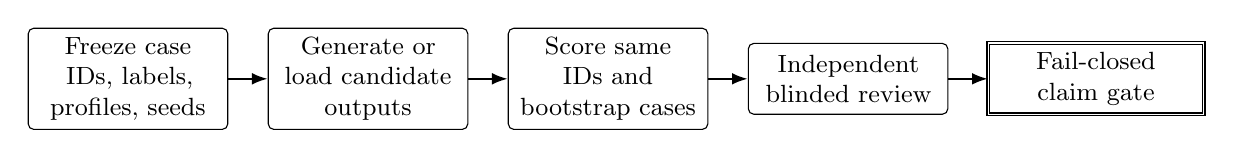
\begin{tikzpicture}[
  node distance=6mm and 5mm,
  box/.style={draw, rounded corners=2pt, align=center, minimum height=9mm, text width=23mm, font=\small},
  gate/.style={draw, double, align=center, minimum height=9mm, text width=25mm, font=\small},
  arrow/.style={-{Latex[length=2mm]}, thick}
]
\node[box] (freeze) {Freeze case IDs, labels, profiles, seeds};
\node[box, right=of freeze] (predict) {Generate or load candidate outputs};
\node[box, right=of predict] (score) {Score same IDs and bootstrap cases};
\node[box, right=of score] (review) {Independent blinded review};
\node[gate, right=of review] (claim) {Fail-closed claim gate};
\draw[arrow] (freeze) -- (predict);
\draw[arrow] (predict) -- (score);
\draw[arrow] (score) -- (review);
\draw[arrow] (review) -- (claim);
\end{tikzpicture}
\caption{Benchmark protocol. Scoring completion alone does not authorize a
broad claim; review status is a separate machine-checked gate.}
\label{fig:protocol}
\end{figure*}


\section{Experiments}
The frozen full run evaluates ContextTrace-Diag-150, a 200-case RAGTruth subset,
and same-ID baseline outputs. Table~\ref{tab:table1-main-results} reports dataset-level
metrics and confidence intervals; Table~\ref{tab:table2-baselines} limits comparisons
to shared outputs. These numbers are pre-review and are not paper-result
eligible until the independent annotation gates pass.

% Generated by paper/generate_tables.py; do not edit manually.
\begin{table*}[t]
\centering
\scriptsize
\resizebox{\textwidth}{!}{%
\begin{tabular}{llllllll}
\toprule
 Dataset & Review status & Cases & Failure F1 & Root cause & Citation F1 & Span overlap & False green \\
\midrule
 RAGTruth & assisted\_review\_pending\_independent & 200 & 0.955 & 0.955 & 1.000 & 0.786 & 0.000 \\
 ContextTrace-Diag-150 & pending\_independent & 150 & 1.000 & 1.000 & 1.000 & 0.950 & 0.000 \\
\bottomrule
\end{tabular}%
}
\caption{Table1 Main Results. Review status and unavailable measurements are shown explicitly.}
\label{tab:table1-main-results}
\end{table*}

% Generated by paper/generate_tables.py; do not edit manually.
\begin{table*}[t]
\centering
\scriptsize
\resizebox{\textwidth}{!}{%
\begin{tabular}{lllllllll}
\toprule
 System & Review status & Cases & Failure F1 & Claim F1 & Root cause & Citation F1 & Span overlap & False green \\
\midrule
 ContextTrace & assisted\_review\_pending\_independent & 200 & 0.955 & 0.337 & 0.955 & 1.000 & 0.786 & 0.000 \\
 RAGAS & same-ID cached baseline & 200 & 0.152 & 0.533 & N/A & N/A & N/A & 0.300 \\
\bottomrule
\end{tabular}%
}
\caption{Table2 Baselines. Review status and unavailable measurements are shown explicitly.}
\label{tab:table2-baselines}
\end{table*}


\section{Ablations}
We disable one diagnostic capability at a time where the implementation permits
a controlled comparison. Lexical-only and semantic-only modes retain only their
named matcher. Two requested model-dependent variants are unavailable under the
frozen offline contract and are reported as such. Table~\ref{tab:table3-ablations}
contains all eleven registered rows.

% Generated by paper/generate_tables.py; do not edit manually.
\begin{table*}[t]
\centering
\scriptsize
\resizebox{\textwidth}{!}{%
\begin{tabular}{llllllllll}
\toprule
 Variant & Availability & Review status & Failure F1 & Root cause & Citation F1 & Span overlap & False green & p95 ms & Cost / 100 \\
\midrule
 Full ContextTrace & available & engineering regression benchmark & 1.000 & 1.000 & 1.000 & 0.862 & 0.000 & 38.978 & 0.000 \\
 Lexical-only verifier & available & engineering regression benchmark & 0.419 & N/A & N/A & N/A & 0.232 & 3.366 & 0.000 \\
 Semantic-only verifier & available & engineering regression benchmark & 0.419 & N/A & N/A & N/A & 0.232 & 20.541 & 0.000 \\
 No citation module & available & engineering regression benchmark & 0.831 & 0.878 & N/A & 0.862 & 0.122 & 36.000 & 0.000 \\
 No contradiction checks & available & engineering regression benchmark & 0.812 & 0.980 & 1.000 & 0.862 & 0.008 & 41.366 & 0.000 \\
 No abstention logic & available & engineering regression benchmark & 0.875 & 0.372 & 1.000 & 0.862 & 0.000 & 38.715 & 0.000 \\
 No root-cause classifier & available & engineering regression benchmark & 1.000 & N/A & 1.000 & 0.862 & 0.000 & 45.393 & 0.000 \\
 No source trust/freshness & available & engineering regression benchmark & 0.708 & 0.888 & 1.000 & 0.862 & 0.112 & 17.151 & 0.000 \\
 No evidence-span localization & available & engineering regression benchmark & 0.982 & 0.998 & 1.000 & N/A & 0.000 & 57.817 & 0.000 \\
 NLI-only mode & not\_available & engineering regression benchmark & N/A & N/A & N/A & N/A & N/A & N/A & N/A \\
 Judge-only mode & not\_available & engineering regression benchmark & N/A & N/A & N/A & N/A & N/A & N/A & N/A \\
\bottomrule
\end{tabular}%
}
\caption{Table3 Ablations. Review status and unavailable measurements are shown explicitly.}
\label{tab:table3-ablations}
\end{table*}


\section{RQ4: Diagnosis Actionability}
RQ4 asks whether evidence-chain diagnoses help humans identify a concrete
repair. The preregistered paired study compares a semantic-core output with the
full evidence-chain output on 40 stratified failure cases, using at least three
non-author reviewers. Primary and secondary outcomes, blinding limits, and
analysis rules are frozen before responses are collected.

No human responses or controlled simulated-pilot outputs are present in this
snapshot. Table~\ref{tab:table4-rq4-actionability} therefore reports N/A and pending status, and
Figure~\ref{fig:rq4} documents the evaluation settings without implying an
outcome.

% Generated by paper/generate_tables.py; do not edit manually.
\begin{table*}[t]
\centering
\scriptsize
\resizebox{\textwidth}{!}{%
\begin{tabular}{llllllll}
\toprule
 Study & Review status & Cases & Reviewers / agents & Root cause & Fix proxy & Actionability & False green \\
\midrule
 Preregistered paired actionability study & pending three independent reviewers & 40 & 0/3 humans & N/A & N/A & N/A & N/A \\
 Simulated A: raw trace & LLM-simulated pilot; not human validation & 40 & 3 & 0.067 & 0.008 & 3.767 & 0.625 \\
 Simulated B: score only & LLM-simulated pilot; not human validation & 40 & 3 & 0.117 & 0.017 & 3.608 & 0.550 \\
 Simulated C: evidence chain & LLM-simulated pilot; not human validation & 40 & 3 & 0.908 & 0.342 & 3.333 & 0.400 \\
\bottomrule
\end{tabular}%
}
\caption{Table4 Rq4 Actionability. Review status and unavailable measurements are shown explicitly.}
\label{tab:table4-rq4-actionability}
\end{table*}

\begin{figure}[t]
\centering
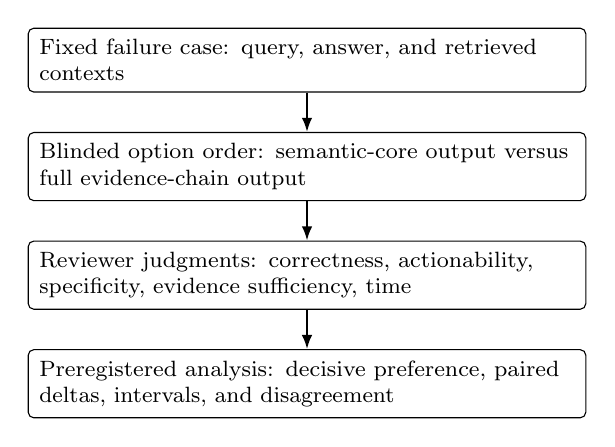
\begin{tikzpicture}[
  node distance=5mm,
  item/.style={draw, rounded corners=2pt, align=left, text width=68mm, font=\footnotesize, inner sep=4pt},
  arrow/.style={-{Latex[length=1.8mm]}, thick}
]
\node[item] (case) {Fixed failure case: query, answer, and retrieved contexts};
\node[item, below=of case] (options) {Blinded option order: semantic-core output versus full evidence-chain output};
\node[item, below=of options] (ratings) {Reviewer judgments: correctness, actionability, specificity, evidence sufficiency, time};
\node[item, below=of ratings] (analysis) {Preregistered analysis: decisive preference, paired deltas, intervals, and disagreement};
\draw[arrow] (case) -- (options);
\draw[arrow] (options) -- (ratings);
\draw[arrow] (ratings) -- (analysis);
\end{tikzpicture}
\caption{RQ4 study settings. The protocol is frozen; responses have not yet
been collected.}
\label{fig:rq4}
\end{figure}


\section{Error Analysis}
The frozen RAGTruth subset contains nine primary-label misses and no dangerous
false-green cases under the current labels. Table~\ref{tab:table5-error-analysis}
separates observed clusters from categories that were not measured or not run.
Examples remain review-pending; the final analysis will incorporate reviewer
corrections without silently changing the frozen case set.

% Generated by paper/generate_tables.py; do not edit manually.
\begin{table*}[t]
\centering
\scriptsize
\resizebox{\textwidth}{!}{%
\begin{tabular}{lllllll}
\toprule
 Cluster & Review status & Count & Example & What happened / likely cause & Planned fix & Affects broad claim \\
\midrule
 Supported claim overflagged & assisted\_review\_pending\_independent & 4 & ragtruth\_9604 & Support threshold or label boundary & Independent adjudication and calibrated claim decomposition & True \\
 Contradiction missed & assisted\_review\_pending\_independent & 2 & ragtruth\_121 & Taxonomy boundary or implicit contradiction & Adjudicate labels; add contradiction regression cases & True \\
 Evidence span too broad & assisted\_review\_pending\_independent & not\_measured & N/A & No dedicated breadth annotation & Add span-boundary error tags during review & unknown \\
 Multi-span evidence failure & assisted\_review\_pending\_independent & not\_measured & N/A & Distributed evidence is not separately tagged & Add multi-span annotations and recall metric & unknown \\
 Root cause confused & assisted\_review\_pending\_independent & 9 & ragtruth\_121 & Failure label and upstream cause are difficult to separate & Adjudicate root causes and report agreement & True \\
 Numeric/date normalization error & assisted\_review\_pending\_independent & not\_measured & N/A & No dedicated numeric/date error tag & Add typed normalization error labels & unknown \\
 Citation mismatch ambiguity & assisted\_review\_pending\_independent & 0 & N/A & No citation mismatch was observed in the primary errors & Retain citation-specific regression coverage & False \\
 Stale/source-trust limitation & assisted\_review\_pending\_independent & not\_measured & N/A & RAGTruth does not independently label source freshness & Evaluate on a temporally labeled dataset & unknown \\
 Score-only baseline false-green & same-ID cached baseline & 60 & aggregate & Score-only output lacks diagnostic coverage & Report same-ID false-green rate and N/A fields & True \\
 Judge parse failure & not\_run & not\_run & N/A & Judge-only mode is unavailable without a frozen provider & Pin provider/model/cache/cost before running & unknown \\
\bottomrule
\end{tabular}%
}
\caption{Table5 Error Analysis. Review status and unavailable measurements are shown explicitly.}
\label{tab:table5-error-analysis}
\end{table*}


\section{Discussion}
The present evidence supports a narrower claim than broad state of the art:
ContextTrace is a reproducible, local-first evidence-chain forensic system with
strong pre-review performance on the frozen failure-label protocol. Claim-level
verdict performance is weaker than the matched baseline on RAGTruth, and the
systems expose different diagnostic coverage. Independent review and RQ4 are
therefore decision-critical rather than procedural formalities.

% Generated by paper/generate_tables.py; do not edit manually.
\begin{table*}[t]
\centering
\scriptsize
\resizebox{\textwidth}{!}{%
\begin{tabular}{llll}
\toprule
 Item & Review status & Value & Status \\
\midrule
 Source revision & pre\_review\_paper\_candidate & 15cf09f9f9d7bfdd6285dae2603edad12d8a3ff9 & frozen \\
 Command & pre\_review\_paper\_candidate & python benchmarks/contexttrace\_bench/reproduce\_arr\_tables.py --full --output-dir 'benchmarks\textbackslash{}contexttrace\_bench\textbackslash{}out\textbackslash{}arr\_full' & full \\
 Python & pre\_review\_paper\_candidate & 3.8.10 & recorded \\
 Runtime seconds & pre\_review\_paper\_candidate & 249.847 & recorded \\
 Bootstrap & pre\_review\_paper\_candidate & 400 / 20260612 & frozen \\
 ContextTrace API cost & pre\_review\_paper\_candidate & 0.0 & local \\
 Candidate cost & same-ID cached baseline & N/A & cached/unreported \\
 Paper result eligible & pending independent review & False & pending review \\
\bottomrule
\end{tabular}%
}
\caption{Table6 Reproducibility. Review status and unavailable measurements are shown explicitly.}
\label{tab:table6-reproducibility}
\end{table*}


\section{Conclusion}
ContextTrace turns RAG traces into inspectable claim, evidence, citation, and
root-cause records. The implementation and frozen experiment pipeline are
complete enough for independent audit, but the paper remains pre-review. The
next evidence milestone is external sign-off followed by the preregistered
actionability study.

\section{Limitations}
Current quantitative results are not independently signed off. The diagnostic
benchmark contains synthetic cases, while the external evaluation uses a
restricted sample rather than every available record. RAGTruth claim-verdict
performance is substantially lower than its failure-label score. Some modules
depend on metadata that real traces may omit. The lexical and semantic matchers
are deterministic heuristics, not general entailment models. NLI-only and
judge-only ablations are unavailable because no offline, version-pinned models
were frozen. The RQ4 study has not been run, and its paired outputs cannot fully
blind reviewers to which condition is more detailed. Grounding against supplied
contexts does not establish real-world truth.

\section{Ethics Statement}
The system evaluates supplied traces and can run locally, reducing the need to
send potentially sensitive prompts or retrieved documents to third parties.
Users remain responsible for dataset licenses, access controls, retention, and
human-subjects requirements. Diagnostic scores should not be used as sole
evidence for high-stakes deployment decisions. Human-study participation must
be voluntary, appropriately reviewed where required, and reported without
identifying reviewers in the anonymous submission.


\bibliographystyle{acl_natbib}
\bibliography{references}
\end{document}
